% Loc-Camlel-Route: Scientific Project Documentation
\documentclass[11pt,a4paper]{article}
\usepackage[margin=1in]{geometry}
\usepackage{graphicx}
\usepackage{tikz}
\usepackage{hyperref}
\usepackage{longtable}
\usepackage{array}
% Remove duplicated tikz package
% \usepackage{tikz}
\usetikzlibrary{positioning,calc}
\title{Loc-Camel-Route}
\author{Alberto Espinosa (KS-Group)}
\date{Oct 19th, 2025}
\begin{document}
\maketitle
\begin{abstract}
This document describes a contract-first, BPEL-driven integration sample and its transformation into a Spring + Maven + Camel implementation using local agentic tooling. It clarifies the problem, the original technology stack and artefacts, the proposed agent architecture and information flow, and the expected results. It also defines project organisation and installation scripts required to run the pipeline without mocks, using only real endpoints and data.
\end{abstract}


\section{Problem Statement}
The sample contains SOAP (Simple Object Access Protocol: XML-based messaging protocol for web services) WSDL (Web Services Description Language: XML format describing service interfaces)/XSD (XML Schema Definition: XML format defining data structures) contracts and a BPEL (Business Process Execution Language: XML language for orchestrating web-service workflows) process \emph{(LocationRetrievalLOC3X1Process)} that orchestrates two inbound operations and multiple partner service calls. There is no runnable Java build, no proper server host, and legacy Java snippets are considered non-authoritative. The problem is to translate this into a robust Spring Boot (Java micro-service framework) + Maven (Java build/dependency tool) project with Apache Camel (integration routing engine)/CXF (Java web-service framework), regenerate models and stubs from contracts, implement deterministic mappings that replace BPEL assignments, externalise configuration, and provide contract and integration verification. The transformation must be automated by local agents and verified end-to-end without mocks; integration results depend on live endpoints.

\section{Original Technology and Artefacts}
\subsection{Overview}
The original sample is contract-first and IBM BPEL-centric:
\begin{itemize}
  \item WSDL/XSD defining document/literal SOAP operations for Location and Country services.
  \item BPEL process (IBM WebSphere style) with partner links, variables, fault handlers, and embedded Java logging/fault composition.
  \item HTTP binding WSDLs referencing localhost endpoints.
  \item Shared fault schema (SimpleFault.xsd).
\end{itemize}
\subsection{Organisation Diagram}

Figure \ref{fig:org-diagram} illustrates the folder organisation of the original sample.

\begin{figure}[h]
\centering
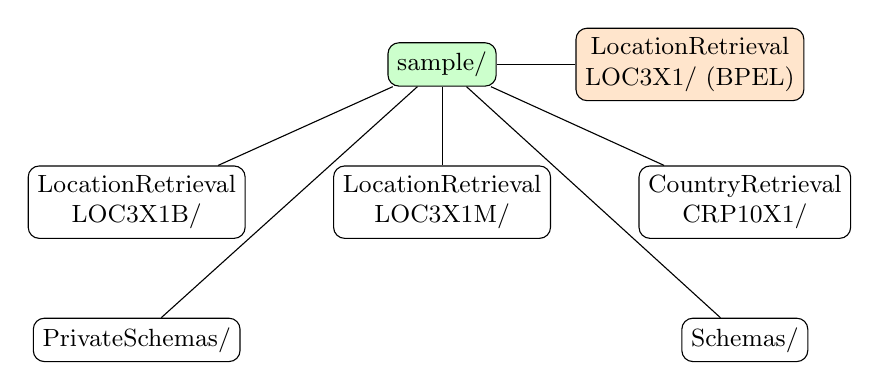
\begin{tikzpicture}[node distance=1.6cm, every node/.style={draw, rectangle, rounded corners, align=center, font=\small}]
\node (root) [fill=green!20] {sample/};
\node (locb) [below left=1.0cm and 1.8cm of root] {LocationRetrieval\\LOC3X1B/};
\node (locm) [below=1.0cm of root] {LocationRetrieval\\LOC3X1M/};
\node (country) [below right=1.0cm and 1.8cm of root] {CountryRetrieval\\CRP10X1/};
\node (bpel) [right=1.0cm of root, fill=orange!20] {LocationRetrieval\\LOC3X1/ (BPEL)};
\node (priv) [below=1.0cm of locb] {PrivateSchemas/};
\node (schemas) [below =1.0cm of country] {Schemas/};
\draw (root) -- (locb);
\draw (root) -- (locm);
\draw (root) -- (country);
\draw (root) -- (priv);
\draw (root) -- (schemas);
\draw (bpel) -- (root);
\end{tikzpicture}
\caption{Folder organisation of the original sample.}\label{fig:org-diagram}
\end{figure}


\section{File Structure and Standards}
\subsection{Summary Table}

Table \ref{tab:file-structure} summarises the key folders and files, their types, and roles.

\renewcommand{\arraystretch}{1.2}
\begin{longtable}{|>{\raggedright\arraybackslash}p{3.5cm}|>{\raggedright\arraybackslash}p{3.2cm}|>{\raggedright\arraybackslash}p{7.2cm}|}
\caption{File structure summary of the original sample.}\label{tab:file-structure}\\
\hline
\textbf{Folder/File} & \textbf{Type} & \textbf{Role} \\
\hline
LocationRetrieval LOC3X1 / LocationRetrieval LOC3X1Process.bpel & BPEL & Orchestration: pick/onMessage for inbound operations, partner links (LOC3X1M, CRP11X1, CRP10X1), variables, fault handlers, logging. \\
\hline
LocationRetrieval LOC3X1B / LocationRetrievalLOC3X1B.wsdl & WSDL & Public interface: LOC3X1B operations, request/response messages, faults. \\
\hline
LocationRetrieval LOC3X1M / LocationRetrievalLOC3X1M.wsdl & WSDL & Internal interface: LOC3X1M operations to which requests are transformed. \\
\hline
CountryRetrieval CRP10X1 / CountryRetrievalCRP10X1.wsdl & WSDL & Partner interface: country retrieval operation(s). \\
\hline
PrivateSchemas / SimpleFault.xsd & XSD & Shared fault structure (FaultMessageText). \\
\hline
Schemas/* & XSD & Domain types referenced by requests/replies across services. \\
\hline
\end{longtable}
\paragraph*{File types: functions, protocols, and standards}
\begin{itemize}
  \item \textbf{BPEL (Business Process Execution Language)}: Defines executable orchestration of service interactions (picks, onMessage, invoke, assign, fault handlers). It runs on a BPEL engine and coordinates partner links and variables to implement business processes, typically calling SOAP-based services described by WSDL. Common deployment uses HTTP(S) transport and adheres to vendor-specific extensions (e.g., IBM WebSphere styles) while following WS-BPEL principles.
  \item \textbf{WSDL (Web Services Description Language)}: Specifies service contracts, including operations (portTypes), request/response messages, bindings, and service endpoints. In this sample WSDLs are document/literal SOAP with HTTP(S) bindings and include fault definitions. Good practice is alignment with WS-I Basic Profile and consistent namespaces and versions for cross-service compatibility.
  \item \textbf{XSD (XML Schema Definition)}: Provides formal XML type definitions for messages and domain objects used by WSDL services and BPEL variables. XSDs enforce structure and validation, carry namespaces for modularity, and support versioning. The shared SimpleFault.xsd standardises fault payloads across services, enabling consistent error reporting.
\end{itemize}


\section{Project Description}
\subsection{Objectives}
Create an automated, agent-driven translation from BPEL + contracts into a Spring Boot + Maven project using Camel/CXF, with deterministic mappings and centralised fault handling, verified via contract checks and real integration tests.

\subsection{Feasibility and Importance}
Feasibility is high because the assets are contract-first and the BPEL encodes mediation steps. Importance lies in replacing legacy BPEL with modern Java micro-integration while preserving behaviour, improving maintainability, and enabling reproducible automation.

\subsection{Challenges and Fine Points}
IBM-specific BPEL features (BOFactory, SDO) must be mapped to plain JAXB + Spring. Some imports may be missing, and business rule nodes (e.g., fire district checks) require explicit specifications. End-to-end tests depend on live partner endpoints; when unavailable, tests must be reported as blocked, never simulated.

\subsection{Used Technology}
\begin{itemize}
  \item \textbf{Deterministic agents via shell/Python; optional LLM reviewer (Ollama/LangGraph)} — Reproducible, CI-safe automation core with an optional, explainability-only reviewer.
  \item \textbf{Java 17} — Long-term-support JVM release providing modern language features and performance.
  \item \textbf{Maven} — Declarative Java build and dependency-management tool.
  \item \textbf{Spring Boot} — Opinionated micro-service framework for rapid, production-ready Spring applications.
  \item \textbf{Apache Camel} — Enterprise-integration patterns engine for declarative routing and mediation.
  \item \textbf{Apache CXF} — Open-source services framework supporting JAX-WS/JAX-RS and SOAP/REST bindings.
  \item \textbf{JAXB/JAX-WS tooling} — Standard XML binding and web-service stub generation from WSDL/XSD.
  \item \textbf{MapStruct} — Compile-time code generator for type-safe, high-performance object mappings.
  \item \textbf{SLF4J/Logback} — Simple logging façade with fast, configurable log implementation.
  \item \textbf{JUnit} — Ubiquitous testing framework for unit and integration verification.
  \item \textbf{Shell/Python automation drivers} — Portable scripts executed inside the project virtual environment to drive agent workflows.
  \item \textbf{jq/yq} — CLI tools for JSON/YAML processing used by contract discovery and preflight reporting.
  \item \textbf{Docker \/ Docker Compose} — Containerisation of services, clients, orchestration, FastAPI, and optional DB; local multi-service orchestration.
  \item \textbf{CI\/CD (GitHub Actions or Jenkins)} — Deterministic pipeline executing preflight, build, test, packaging, and container publish.
  \item \textbf{Node.js \/ React} — Frontend dashboard for evidence browsing and orchestration controls.
  \item \textbf{Python \/ FastAPI} — Lightweight API for evidence metadata and agent orchestration hooks.
\end{itemize}

\subsection{Local Models via Ollama}
\begin{itemize}
  \item Reviewer/Interpreter model (optional): runs after evaluation to generate an executive explanation report from artefacts; never changes code or gates release.
  \item Deterministic core: planning, scaffolding, build, tests, evaluation executed by shell/Python without LLM; reproducible and CI-safe.
  \item Retrieval (optional): embeddings used solely to fetch relevant artefact snippets for the reviewer; not required for the core.
\end{itemize}
Table \ref{tab:local-models} details the optional reviewer model and supporting components when enabled.
\renewcommand{\arraystretch}{1.2}
\begin{longtable}{|>{\raggedright\arraybackslash}p{3.2cm}|>{\raggedright\arraybackslash}p{6.0cm}|>{\raggedright\arraybackslash}p{6.0cm}|}
\caption{Recommended local models and rationale.}\label{tab:local-models}\\
\hline
\textbf{Model Role} & \textbf{Recommended Model(s)} & \textbf{Rationale} \\
\hline
Instruction / Planner & Llama 3 Instruct (local) & Strong instruction-following aids planning, decomposition, and policy adherence (no mocks, British English), producing reliable agent steps and acceptance criteria. \\
\hline
Code Generation & CodeLlama or Qwen Coder (local) & Trained for programming tasks; produces idiomatic Java, Spring Boot, Maven, Camel, and CXF code with fewer syntax errors and better library usage patterns. \\
\hline
Embedding / Retrieval & nomic-embed-text or mxbai-embed-large (local) & High-quality embeddings for contract/code search, enabling deterministic mapping between WSDL/XSD schemas and generated classes, improving route wiring accuracy. \\
\hline
\end{longtable}


\subsection{Agentic System Architecture}
Agents: Planner, Contract Reader, BPEL Parser, Schema Aligner, Integration Builder (CXF/Camel), Mapping Builder (MapStruct), Test Designer, Environment Installer, Evaluator/Referee. Each agent has a focused remit and produces artefacts consumed downstream.

% Emphasise Environment Installer responsibilities
The Environment Installer performs a tooling preflight, verifies JDK/Maven and auxiliary tools (jq/yq, Python packages), installs missing dependencies where permitted, and emits a versioned readiness report at \texttt{doc/tooling-report.md}. It ensures all downstream agents can compile, run, capture logs, and evaluate correctness.

Figure \ref{fig:agent-pipeline} presents the agentic system pipeline, congruent with Table \ref{tab:agent-summary}. Figure \ref{fig:bpel-flow} depicts the high-level mediation flow derived from BPEL.

\begin{figure}[ht]
\centering
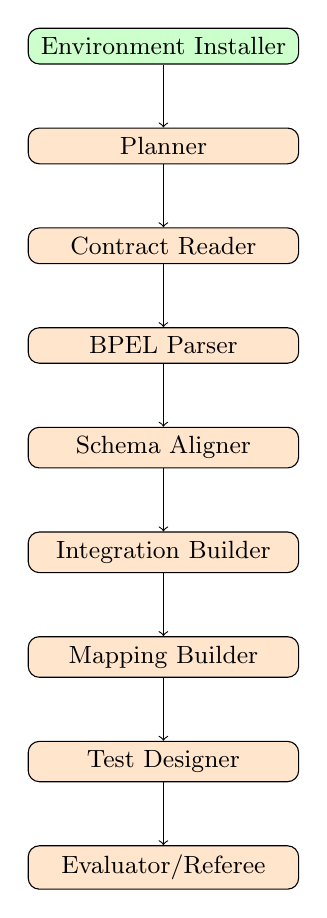
\begin{tikzpicture}[node distance=0.8cm, every node/.style={draw, rectangle, rounded corners, align=center, font=\small, text width=3.2cm}]
\node (env) [fill=green!20] {Environment Installer};
\node (plan) [below=of env, fill=orange!20] {Planner};
\node (contract) [below=of plan, fill=orange!20] {Contract Reader};
\node (bpel) [below=of contract, fill=orange!20] {BPEL Parser};
\node (schema) [below=of bpel, fill=orange!20] {Schema Aligner};
\node (integration) [below=of schema, fill=orange!20] {Integration Builder};
\node (mapping) [below=of integration, fill=orange!20] {Mapping Builder};
\node (test) [below=of mapping, fill=orange!20] {Test Designer};
\node (eval) [below=of test, fill=orange!20] {Evaluator/Referee};

\draw[->] (env) -- (plan);
\draw[->] (plan) -- (contract);
\draw[->] (contract) -- (bpel);
\draw[->] (bpel) -- (schema);
\draw[->] (schema) -- (integration);
\draw[->] (integration) -- (mapping);
\draw[->] (mapping) -- (test);
\draw[->] (test) -- (eval);
\end{tikzpicture}
\caption{Agentic system pipeline congruent with the summary table.}\label{fig:agent-pipeline}
\end{figure}

\begin{figure}[h]
\centering
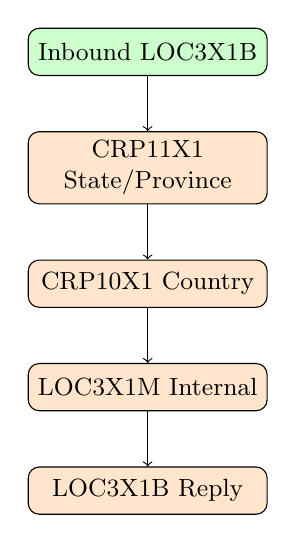
\begin{tikzpicture}[node distance=0.7cm, every node/.style={draw, rectangle, rounded corners, align=center, font=\small, text width=2.8cm, minimum height=0.6cm}]
\node (in) [fill=green!20] {Inbound LOC3X1B};
\node (state) [below=of in, fill=orange!20] {CRP11X1 State/Province};
\node (country) [below=of state, fill=orange!20] {CRP10X1 Country};
\node (locm) [below=of country, fill=orange!20] {LOC3X1M Internal};
\node (out) [below=of locm, fill=orange!20] {LOC3X1B Reply};
\draw[->] (in) -- (state);
\draw[->] (state) -- (country);
\draw[->] (country) -- (locm);
\draw[->] (locm) -- (out);
\end{tikzpicture}
\caption{High-level flow derived from BPEL mediation.}\label{fig:bpel-flow}
\end{figure}


\renewcommand{\arraystretch}{1.2}
\begin{table}[ht]
\centering
\renewcommand{\arraystretch}{1.2}
\caption{Agent responsibilities, inputs, and outputs.}\label{tab:agent-summary}
\begin{tabular}{|>{\raggedright\arraybackslash}p{3cm}|>{\raggedright\arraybackslash}p{6cm}|>{\raggedright\arraybackslash}p{3.5cm}|>{\raggedright\arraybackslash}p{3.5cm}|}
\hline
\textbf{Agent} & \textbf{Responsibility} & \textbf{Inputs} & \textbf{Outputs} \\
\hline
Planner & Global plan, dependency ordering, acceptance criteria alignment & BPEL, WSDL/XSD inventory & Execution plan, module breakdown \\
\hline
Contract Reader & Generate JAXB/CXF artefacts and validate contracts & WSDL/XSD & Models, stubs, contract validation report \\
\hline
BPEL Parser & Extract inbound ops, partner invocations, variables, fault logic & BPEL & Orchestration spec, mapping intents \\
\hline
Schema Aligner & Namespace/version governance and schema catalogue curation & XSD set & Canonical schema map, alignment report \\
\hline
Integration Builder & Configure CXF endpoints and Camel routes & Orchestration spec, properties & Running inbound service, route definitions \\
\hline
Mapping Builder & Deterministic request/response transformations & Orchestration spec, models & Mapper implementations and tests \\
\hline

\hline
Environment Installer & Provision local JDK/Maven and project tooling & Script definitions & Installed toolchain, verified versions \\
\hline
Evaluator/Referee & Verify builds, runtime, tests; produce final audit & Build outputs, test reports & Evaluation summary, blockers list \\
\hline
\end{tabular}
\end{table}



\subsection{Expected Results}
A runnable Spring Boot application exposing LOC3X1B operations; generated CXF clients for partners; mappings that mirror BPEL assignments; centralised fault handling producing SimpleFault; contract validations passing; integration tests either passing against live endpoints or clearly reported as blocked.

\textit{Note: The orchestration specification includes a \texttt{data\_mappings} section derived deterministically by parsing original IBM \texttt{.map} XML artefacts (e.g., \texttt{map:businessObjectMap} and \texttt{map:propertyMap}). This reflects IBM BPEL script-based transformations rather than \texttt{bpws:assign} elements.}

\section{Project Organisation}
Recommended directory layout (generalised monorepo):

\begin{verbatim}
project-root/
|-- doc/                # LaTeX, tickets, plans, reports
|-- scripts/            # Automation (preflight, build, run, tests, test_master)
|-- contracts/          # Inventories, canonical maps, generated artefacts
|-- modules/            # Maven multi-module: contracts, services/loc3x1b, clients/{loc3x1m,crp11x1,crp10x1}, mappings, orchestration, tests
|-- docker/             # Dockerfiles and docker-compose.yml
|-- api/                # FastAPI service (evidence, orchestration endpoints)
`-- tests/              # Test artefacts and JUnit XML outputs (mirrors sections)
\end{verbatim}

\section{Installation Scripts (Definition)}
\begin{itemize}
  \item \texttt{scripts/preflight.sh} – Runs tooling preflight, verifies JDK/Maven and CLI tools, produces \texttt{doc/tooling-report.md}, and attempts a smoke build if a Maven project is present.
  \item \texttt{scripts/bootstrap\_java.sh} – Installs JDK and Maven locally so the build toolchain is ready.
  \item \texttt{scripts/generate\_contracts.sh} – Runs JAXB/CXF codegen to create Java models and service stubs from WSDL/XSD.
  \item \texttt{scripts/build\_all.sh} – Executes Maven compile, test and package for the entire project.
  \item \texttt{scripts/run\_services.sh} – Starts the Spring-Boot inbound application exposing the LOC3X1B service.
  \item \texttt{scripts/test\_integrations.sh} – Runs integration tests against live partner endpoints (no mocks).
  \item \texttt{scripts/test\_master.sh} – Master test runner to execute unit tests by ordinal (LOC-XXX), by section, or all.
\end{itemize}
All scripts run inside the project virtual environment for consistent orchestration.

\section{Agentic Strategy and Implementation Philosophy}
\subsection{Overview of the Agentic Approach}
The transformation from BPEL-based integration to modern Spring Boot + Camel architecture employs an \emph{agentic strategy} that fundamentally differs from traditional code generation or manual migration approaches. Rather than producing static artefacts that become obsolete when contracts change, this system implements a \textbf{closed-loop, evidence-driven integration layer} that continuously adapts to evolving service landscapes whilst maintaining operational stability and auditability.

The core philosophy centres on \textbf{dynamic resilience over static perfection}. The agentic system prioritises maintaining functional integrations even when partner services change locations, bindings, or schemas, rather than requiring manual intervention for every contract modification. This approach recognises that enterprise integration environments are inherently volatile, with services frequently updated, relocated, or temporarily unavailable.

\subsection{The Closed-Loop Integration Cycle}
The agentic system operates through a continuous seven-phase cycle: \textbf{Discover → Validate → Synthesise → Verify → Harden → Monitor → Adapt}. This cycle ensures that integration behaviour remains consistent whilst the underlying implementation adapts to environmental changes.

Figure \ref{fig:agentic-cycle} illustrates this closed-loop process, showing how each phase feeds into the next whilst maintaining evidence trails for governance and auditability.

\begin{figure}[ht]
\centering
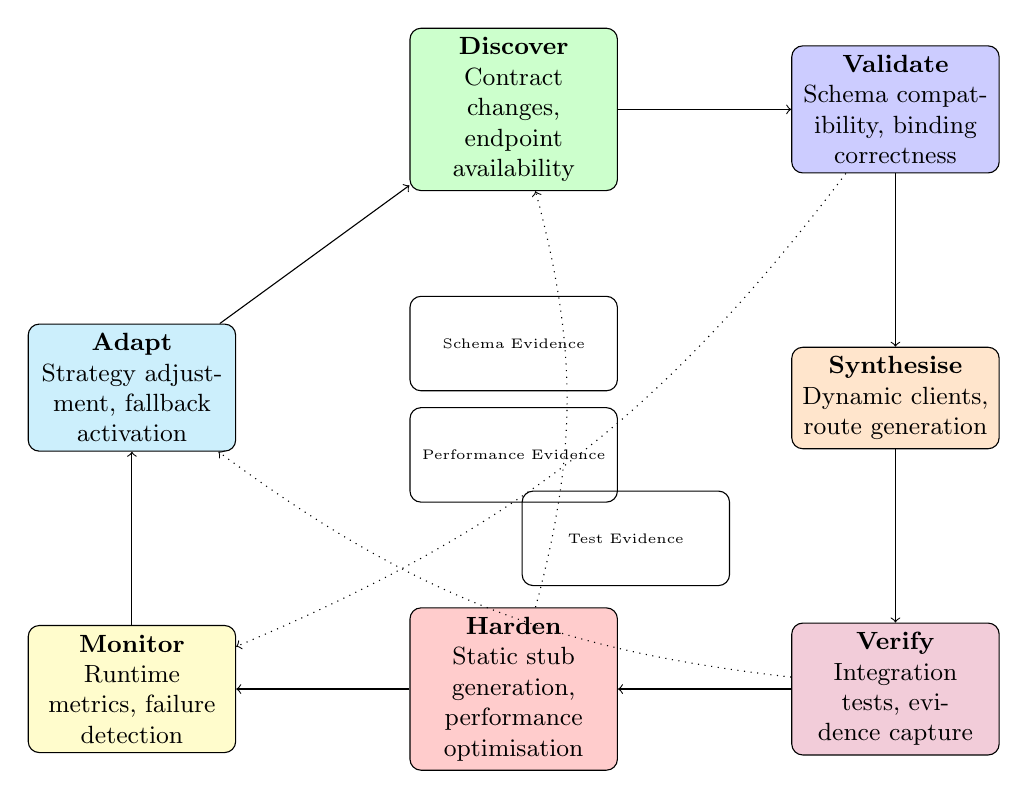
\begin{tikzpicture}[node distance=2.2cm, every node/.style={draw, rectangle, rounded corners, align=center, font=\small, text width=2.4cm, minimum height=1.2cm}]
% Main cycle nodes
\node (discover) [fill=green!20] {\textbf{Discover}\\Contract changes, endpoint availability};
\node (validate) [right=of discover, fill=blue!20] {\textbf{Validate}\\Schema compatibility, binding correctness};
\node (synthesise) [below=of validate, fill=orange!20] {\textbf{Synthesise}\\Dynamic clients, route generation};
\node (verify) [below=of synthesise, fill=purple!20] {\textbf{Verify}\\Integration tests, evidence capture};
\node (harden) [left=of verify, fill=red!20] {\textbf{Harden}\\Static stub generation, performance optimisation};
\node (monitor) [left=of harden, fill=yellow!20] {\textbf{Monitor}\\Runtime metrics, failure detection};
\node (adapt) [above=of monitor, fill=cyan!20] {\textbf{Adapt}\\Strategy adjustment, fallback activation};

% Cycle arrows
\draw[->] (discover) -- (validate);
\draw[->] (validate) -- (synthesise);
\draw[->] (synthesise) -- (verify);
\draw[->] (verify) -- (harden);
\draw[->] (harden) -- (monitor);
\draw[->] (monitor) -- (adapt);
\draw[->] (adapt) -- (discover);

% Evidence flow (dotted lines)
\draw[dotted, ->] (validate) to[bend left=15] (monitor);
\draw[dotted, ->] (verify) to[bend left=15] (adapt);
\draw[dotted, ->] (harden) to[bend right=15] (discover);

% Labels for evidence flows
\node[font=\tiny, above=0.1cm] at ($(validate)!0.5!(monitor)$) {Schema Evidence};
\node[font=\tiny, right=0.1cm] at ($(verify)!0.5!(adapt)$) {Test Evidence};
\node[font=\tiny, below=0.1cm] at ($(harden)!0.5!(discover)$) {Performance Evidence};
\end{tikzpicture}
\caption{The closed-loop agentic integration cycle with evidence flows.}\label{fig:agentic-cycle}
\end{figure}

\subsubsection{Phase Descriptions}
\begin{itemize}
\item \textbf{Discover}: Continuously scans for changes in WSDL locations, schema versions, endpoint availability, and BPEL process definitions. Uses configurable polling intervals and change detection algorithms.
\item \textbf{Validate}: Performs schema compatibility checks, binding validation, and import resolution. Identifies breaking changes versus compatible extensions.
\item \textbf{Synthesise}: Generates integration artefacts using either static code generation (for stable contracts) or dynamic invocation patterns (for volatile contracts). Chooses strategy based on contract stability metrics.
\item \textbf{Verify}: Executes targeted integration tests against live endpoints, capturing evidence of success or failure. Never uses mocks—blocked tests are reported as such.
\item \textbf{Harden}: Converts proven dynamic integrations into optimised static implementations when stability thresholds are met. Maintains both versions during transition periods.
\item \textbf{Monitor}: Tracks runtime performance, error rates, and availability metrics. Detects degradation patterns that trigger cycle re-entry.
\item \textbf{Adapt}: Adjusts integration strategies based on accumulated evidence. May switch from static to dynamic approaches or activate fallback mechanisms.
\end{itemize}

\subsubsection{Deterministic Core and Reviewer Agent}
The core pipeline is \textbf{deterministic}, repository-aware, and evidence-driven. Planning, scaffolding, build, tests, and evaluation are performed by guarded shell/Python scripts that operate only on explicit artefacts (WSDL/XSD, BPEL, YAML specs), enforce virtual-environment execution, and persist logs and run metadata. This yields reproducibility, auditability, and CI compatibility; no local LLM is required for correctness.

\paragraph{Reviewer/Interpreter (Optional)}
When enabled, a local LLM runs \textit{after} evaluation to interpret artefacts and produce an executive explanation report. Inputs include scaffold/build logs, test results, the agent plan, and route specifications. Outputs are written to `doc/reviewer-report.md` as a plain-English narrative of decisions, evidence chains, and risks. The reviewer never changes code or gates release; it augments explainability only.

\paragraph{Guardrails}
LLM outputs are schema-validated and cross-checked against deterministic artefacts; disagreements are flagged, not auto-applied. The deterministic core remains authoritative regardless of reviewer presence.

\subsection{Static versus Dynamic Invocation Strategy}
The agentic system employs a \textbf{hybrid invocation model} that dynamically selects between static code generation and runtime service discovery based on contract stability and operational requirements.

Figure \ref{fig:invocation-strategy} depicts the decision matrix used to determine the optimal invocation approach for each service integration.

\begin{figure}[ht]
\centering
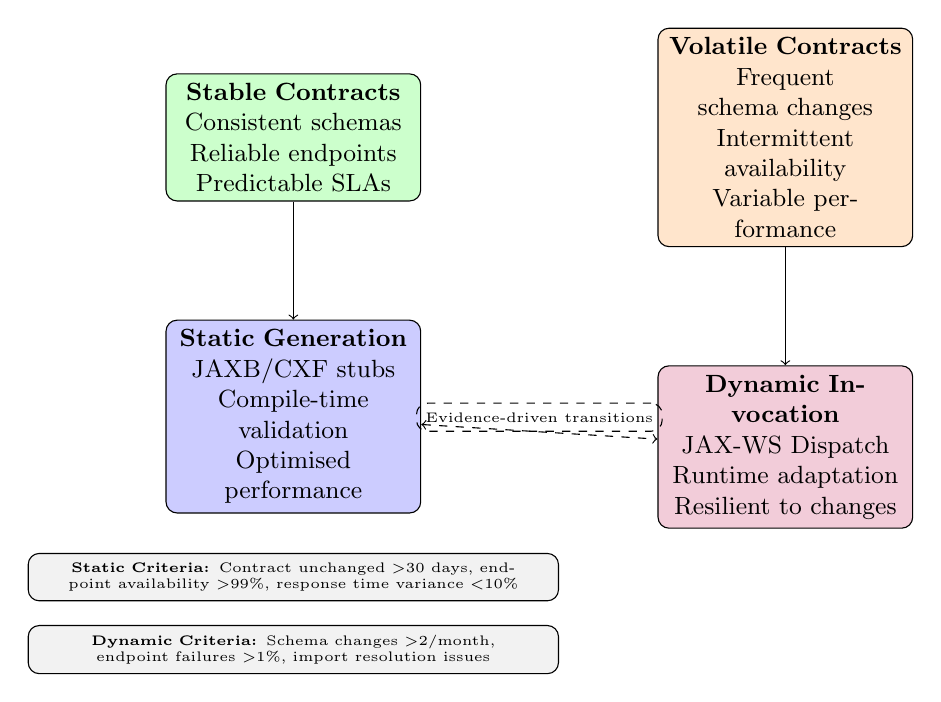
\begin{tikzpicture}[node distance=1.5cm, every node/.style={draw, rectangle, rounded corners, align=center, font=\small}]
% Decision matrix
\node (stable) [fill=green!20, text width=3cm] {\textbf{Stable Contracts}\\Consistent schemas\\Reliable endpoints\\Predictable SLAs};
\node (volatile) [right=3cm of stable, fill=orange!20, text width=3cm] {\textbf{Volatile Contracts}\\Frequent schema changes\\Intermittent availability\\Variable performance};

\node (static) [below=of stable, fill=blue!20, text width=3cm] {\textbf{Static Generation}\\JAXB/CXF stubs\\Compile-time validation\\Optimised performance};
\node (dynamic) [below=of volatile, fill=purple!20, text width=3cm] {\textbf{Dynamic Invocation}\\JAX-WS Dispatch\\Runtime adaptation\\Resilient to changes};

% Decision arrows
\draw[->] (stable) -- (static);
\draw[->] (volatile) -- (dynamic);

% Transition arrows
\draw[<->, dashed] (static) -- (dynamic) node[midway, above, font=\tiny] {Evidence-driven transitions};

% Criteria boxes
\node (criteria1) [below=0.5cm of static, fill=gray!10, text width=6.5cm, font=\tiny] {
\textbf{Static Criteria:} Contract unchanged >30 days, endpoint availability >99\%, response time variance <10\%
};
\node (criteria2) [below=0.3cm of criteria1, fill=gray!10, text width=6.5cm, font=\tiny] {
\textbf{Dynamic Criteria:} Schema changes >2/month, endpoint failures >1\%, import resolution issues
};
\end{tikzpicture}
\caption{Static versus dynamic invocation decision matrix.}\label{fig:invocation-strategy}
\end{figure}

\subsubsection{Static Generation Benefits}
\begin{itemize}
\item \textbf{Performance}: Compile-time optimisation eliminates runtime reflection overhead
\item \textbf{Type Safety}: Strong typing catches integration errors at build time
\item \textbf{IDE Support}: Full code completion and refactoring capabilities
\item \textbf{Debugging}: Stack traces reference actual Java classes rather than dynamic proxies
\end{itemize}

\subsubsection{Dynamic Invocation Benefits}
\begin{itemize}
\item \textbf{Adaptability}: Continues functioning when contracts change without recompilation
\item \textbf{Resilience}: Graceful degradation when endpoints become temporarily unavailable
\item \textbf{Discovery}: Automatic detection of new operations or modified schemas
\item \textbf{Fallback}: Can switch between multiple endpoint versions transparently
\end{itemize}

\subsection{Evidence-Driven Hardening Process}
The transition from dynamic to static implementations follows a rigorous \textbf{evidence-driven hardening process} that ensures stability before committing to optimised static code generation.

\subsubsection{Evidence Collection Metrics}
\begin{itemize}
\item \textbf{Contract Stability}: Time since last schema change, frequency of endpoint modifications
\item \textbf{Operational Reliability}: Success rate, response time consistency, availability percentage
\item \textbf{Integration Complexity}: Number of transformations, fault handling requirements, orchestration depth
\item \textbf{Business Criticality}: SLA requirements, transaction volume, downstream dependencies
\end{itemize}

\subsubsection{Hardening Thresholds}
Static generation is triggered when all of the following criteria are met for a continuous period:
\begin{itemize}
\item Contract unchanged for minimum 30 days
\item Endpoint availability exceeding 99.5\%
\item Response time variance below 10\% of baseline
\item Zero import resolution failures
\item Successful integration test rate above 98\%
\end{itemize}

\subsection{Orchestration Synthesis from BPEL}
The agentic system transforms BPEL orchestration logic into Camel routes through a sophisticated \textbf{orchestration synthesis process} that preserves business logic whilst modernising the execution environment.

Figure \ref{fig:bpel-synthesis} illustrates how BPEL constructs are mapped to equivalent Camel patterns whilst maintaining the original orchestration semantics.

\begin{figure}[ht]
\centering
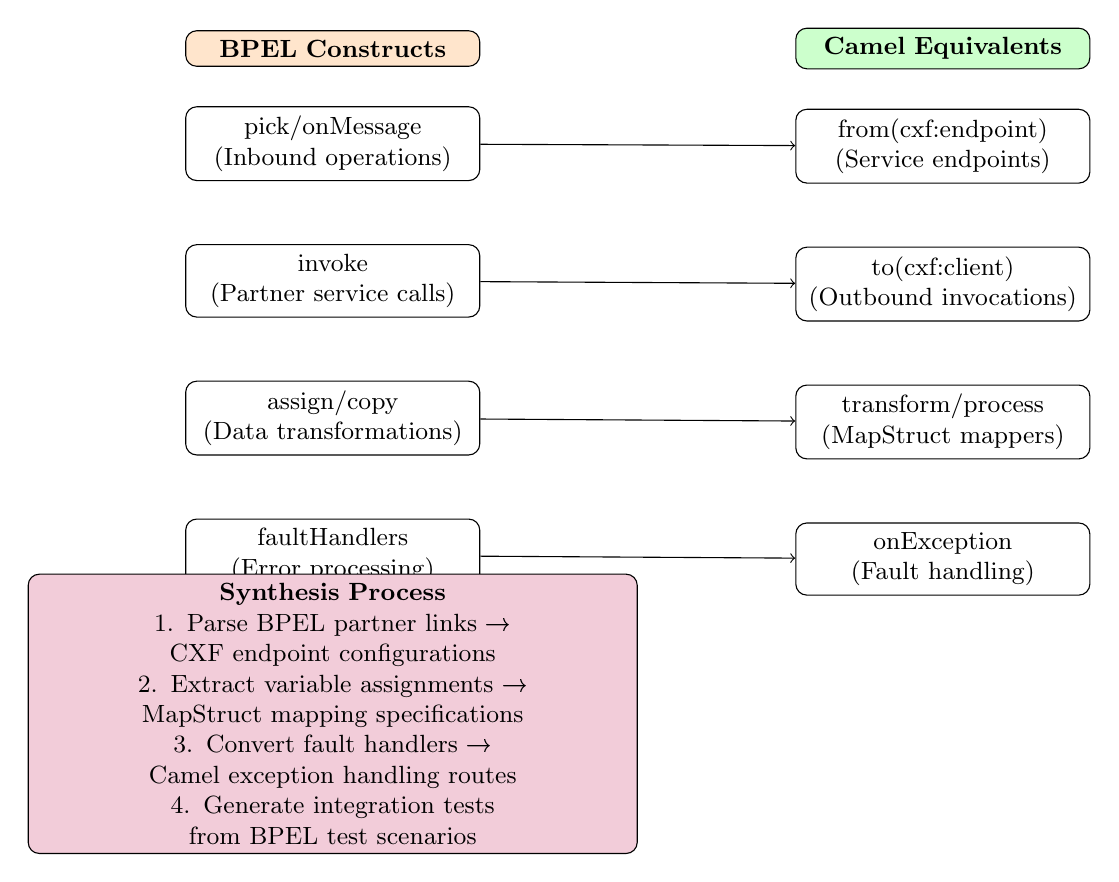
\begin{tikzpicture}[node distance=1.8cm, every node/.style={draw, rectangle, rounded corners, align=center, font=\small}]
% BPEL side
\node (bpel-title) [fill=orange!20, text width=3.5cm] {\textbf{BPEL Constructs}};
\node (pick) [below=0.5cm of bpel-title, text width=3.5cm] {pick/onMessage\\(Inbound operations)};
\node (invoke) [below=0.8cm of pick, text width=3.5cm] {invoke\\(Partner service calls)};
\node (assign) [below=0.8cm of invoke, text width=3.5cm] {assign/copy\\(Data transformations)};
\node (fault) [below=0.8cm of assign, text width=3.5cm] {faultHandlers\\(Error processing)};

% Camel side
\node (camel-title) [right=4cm of bpel-title, fill=green!20, text width=3.5cm] {\textbf{Camel Equivalents}};
\node (from) [below=0.5cm of camel-title, text width=3.5cm] {from(cxf:endpoint)\\(Service endpoints)};
\node (to) [below=0.8cm of from, text width=3.5cm] {to(cxf:client)\\(Outbound invocations)};
\node (transform) [below=0.8cm of to, text width=3.5cm] {transform/process\\(MapStruct mappers)};
\node (exception) [below=0.8cm of transform, text width=3.5cm] {onException\\(Fault handling)};

% Mapping arrows
\draw[->] (pick) -- (from);
\draw[->] (invoke) -- (to);
\draw[->] (assign) -- (transform);
\draw[->] (fault) -- (exception);

% Synthesis process
\node (synthesis) [below=1.5cm of assign, fill=purple!20, text width=7.5cm] {
\textbf{Synthesis Process}\\
1. Parse BPEL partner links → CXF endpoint configurations\\
2. Extract variable assignments → MapStruct mapping specifications\\
3. Convert fault handlers → Camel exception handling routes\\
4. Generate integration tests from BPEL test scenarios
};
\end{tikzpicture}
\caption{BPEL to Camel orchestration synthesis mapping.}\label{fig:bpel-synthesis}
\end{figure}

\subsubsection{Synthesis Algorithms}
\begin{itemize}
\item \textbf{Partner Link Analysis}: Extracts service dependencies and generates corresponding CXF client configurations with appropriate timeout and retry policies
\item \textbf{Variable Flow Tracking}: Maps BPEL variable assignments to type-safe MapStruct transformations, preserving data lineage and validation rules
\item \textbf{Fault Propagation}: Converts BPEL fault handlers into Camel exception handling with appropriate compensation and rollback logic
\item \textbf{Correlation Preservation}: Maintains message correlation patterns from BPEL correlation sets using Camel's correlation identifier mechanisms
\end{itemize}

\subsection{Governance and Safety Mechanisms}
The agentic system incorporates comprehensive \textbf{governance and safety mechanisms} to ensure that automated decisions remain auditable, reversible, and aligned with operational policies.

\subsubsection{Evidence Gates}
Every significant system change must pass through \textbf{evidence gates} that require documented justification and approval criteria:
\begin{itemize}
\item \textbf{Contract Changes}: Schema compatibility analysis, impact assessment, rollback procedures
\item \textbf{Endpoint Modifications}: Availability verification, performance benchmarking, fallback validation
\item \textbf{Route Alterations}: Integration test results, business logic preservation, monitoring coverage
\item \textbf{Hardening Decisions}: Stability evidence, performance improvements, maintenance implications
\end{itemize}

\subsubsection{Auditability Requirements}
All agentic decisions are logged with sufficient detail for post-hoc analysis:
\begin{itemize}
\item \textbf{Decision Context}: Environmental conditions, available evidence, applied policies
\item \textbf{Alternative Considerations}: Other strategies evaluated, rejection rationale
\item \textbf{Implementation Details}: Generated artefacts, configuration changes, test results
\item \textbf{Success Metrics}: Performance improvements, reliability gains, maintenance reductions
\end{itemize}

\subsubsection{Safety Constraints}
The system operates within strict safety boundaries to prevent operational disruption:
\begin{itemize}
\item \textbf{No Secret Exposure}: Credentials and sensitive configuration never logged or committed
\item \textbf{Gradual Rollout}: Changes deployed incrementally with monitoring at each stage
\item \textbf{Automatic Rollback}: Failed changes trigger immediate reversion to last known good state
\item \textbf{Human Override}: Manual intervention capabilities for emergency situations
\end{itemize}

\subsection{Production Operational Model}
In production environments, the agentic system operates as a \textbf{self-healing integration layer} that maintains service continuity whilst adapting to changing conditions.

\subsubsection{Continuous Monitoring}
\begin{itemize}
\item \textbf{Contract Drift Detection}: Automated scanning for WSDL/XSD changes with impact analysis
\item \textbf{Performance Baseline Tracking}: Statistical analysis of response times, throughput, and error rates
\item \textbf{Availability Monitoring}: Endpoint health checks with intelligent retry and circuit breaker patterns
\item \textbf{Integration Quality Metrics}: Success rates, data quality scores, business rule compliance
\end{itemize}

\subsubsection{Adaptive Response Strategies}
When environmental changes are detected, the system employs graduated response strategies:
\begin{enumerate}
\item \textbf{Transparent Adaptation}: Minor changes handled automatically without service interruption
\item \textbf{Graceful Degradation}: Temporary fallbacks activated whilst permanent solutions are synthesised
\item \textbf{Controlled Failover}: Systematic switching to alternative endpoints or service versions
\item \textbf{Emergency Isolation}: Problematic integrations quarantined to prevent cascade failures
\end{enumerate}

\subsubsection{Expected Production Outcomes}
The agentic approach delivers several key operational benefits:
\begin{itemize}
\item \textbf{Reduced Maintenance Overhead}: Automatic adaptation eliminates manual intervention for routine changes
\item \textbf{Improved Reliability}: Multiple fallback strategies and proactive monitoring prevent service disruptions
\item \textbf{Enhanced Visibility}: Comprehensive evidence trails enable rapid problem diagnosis and resolution
\item \textbf{Accelerated Integration}: New services can be integrated rapidly using proven patterns and automated testing
\end{itemize}

This agentic strategy represents a fundamental shift from reactive maintenance to proactive adaptation, enabling integration architectures that evolve gracefully with their operational environments whilst maintaining the reliability and auditability required for enterprise systems.

\section{Conclusion}
The transformation is feasible and valuable. With disciplined agentic automation and strict adherence to the original contracts and BPEL intent, the resulting project will be maintainable, verifiable, and aligned with modern Java integration practices.
\end{document}